\chapter{การทบทวนวรรณกรรมที่เกี่ยวข้อง}
\label{chapter:literature-review}

\section{ปัญหาความไม่สมดุลกันของกลุ่มข้อมูล}
ความไม่สมดุลกันของกลุ่มข้อมูล คือ การที่ตัวอย่างของข้อมูลแต่ละกลุ่มมีจำนวนไม่เท่ากัน และจำนวนตัวอย่างนั้นต่างกันมาก เช่น ชุดข้อมูล A มี 2 กลุ่มข้อมูลจากทั้งหมด 10,500 ตัวอย่าง 
แบ่งออกเป็นกลุ่มข้อมูลที่ 1 จำนวน 500 ตัวอย่าง และกลุ่มข้อมูลที่ 2 จำนวน 10,000 เป็นต้น 

ในงานวิจัย~\cite{Anand:1993} ผู้วิจัยได้ทำการศึกษาเกี่ยวกับผลทระทบของความไม่สมดุลกันของข้อมูลในการเรียนรู้ของแบบจำลอง และพบว่าความไม่สมดุลกันของข้อมูลได้ส่งผลกระทบด้านลบต่อกระบวนการ Backpropagation โดยผลกระทบดังกล่าว คือ การที่กลุ่มข้อมูลส่วนมากมีอิทธิพลต่อค่า Gradient ที่จะถูกนำไปใช้ในการปรับค่า Weight มากกว่ากลุ่มข้อมูลส่วนน้อย เนื่องจากจำนวนตัวอย่างของกลุ่มข้อมูลส่วนมากในแต่ละ Batch ของการเรียนรู้ นั้นมีมากกว่า ทำให้ค่าสูญเสียรวมมีลักษณะที่ค่าสูญของกลุ่มข้อมูลส่วนมากไปกลบค่าสูญเสียของกลุ่มข้อมูลส่วนน้อย 

เหตุการณ์ดังกล่าวทำให้ลักษณะของการเรียนรู้ของแบบจำลองมุ่งไปที่การเรียนรู้เฉพาะกลุ่มข้อมูลส่วนมาก  กล่าวคือ ค่าสูญเสียของกลุ่มข้อมูลส่วนมากจะลดลงอย่างรวดเร็ว ในขณะที่ค่าสูญเสียของกลุ่มข้อมูลส่วนน้อยเพิ่มขึ้นเรื่อย ๆ ในช่วงต้นของการเรียนรู้ สุดท้ายทำให้การเรียนรู้ของแบบจำลองเข้าลู่เข้าจุดที่ดีที่สุดช้าหรือไม่สามารถเรียนรู้ที่จะจัดกลุ่มได้เลย

ความไม่สมดุลกันของกลุ่มข้อมูลนั้นมีอยู่ 2 ประเภท คือ Step Imbalance~\cite{Buda:2017} และ Long-Tailed Imbalance~\cite{Liu:2019} ตามรายละเอียดดังนี้

\begin{itemize}
  \item Step Imbalance เป็นความไม่สมดุลกันของกลุ่มข้อมูลที่จำนวนตัวอย่างของกลุ่มข้อมูลส่วนน้อยแต่ละกลุ่มมีจำนวนเท่ากัน และจำนวนตัวอย่างของกลุ่มข้อมูลส่วนมากแต่ละกลุ่มมีจำนวนเท่ากัน โดยอัตราส่วนของกลุ่มของส่วนน้อยและส่วนมาก ($\mu$) สามารถคำนวณได้จากสมการที่ \ref{eq:stepimbalance} ตัวอย่างการกระจายของจำนวนตัวอย่างของกลุ่มข้อมูลแสดงดังรูปที่ \ref{fig:imb-dist:1} และ \ref{fig:imb-dist:2} 
  \begin{equation}
      \mu = \frac{\left | \left \{ i\in  \left \{ 1,...,N \right \}: C_{i}\:is\:minority\:class \right \} \right |}{N},
      \label{eq:stepimbalance}
    \end{equation}

    โดยที่ $C_{i}$ คือ ชุดของตัวอย่างของกลุ่มข้อมูล $i$ และ N คือ จำนวนกลุ่มตัวอย่างทั้งหมด
  \item Long-Tailed Imbalance เป็นความไม่สมดุลกันของกลุ่มข้อมูลที่จำนวนตัวอย่างของแต่ละกลุ่มข้อมูลมีจำนวนไม่เท่ากันตามตัวอย่างการกระจายของจำนวนตัวอย่างของกลุ่มข้อมูลในรูปที่ \ref{fig:imb-dist:3}
  
\end{itemize}

สามารถคำนวณค่าอัตราส่วนระหว่างจำนวนตัวอย่างของกลุ่มข้อมูลส่วนน้อยและกลุ่มข้อมูลส่วนมาก ($p$) ได้ตามสมการที่ \ref{eq:p_ratio}

\begin{equation}
  p = \frac{max_{i}\left \{ \left | C_{i} \right | \right \}}{min_{i}\left \{ \left | C_{i} \right | \right \}}
  \label{eq:p_ratio}
\end{equation}

\begin{figure}[h]
  \centering
  \subfigure[]{
      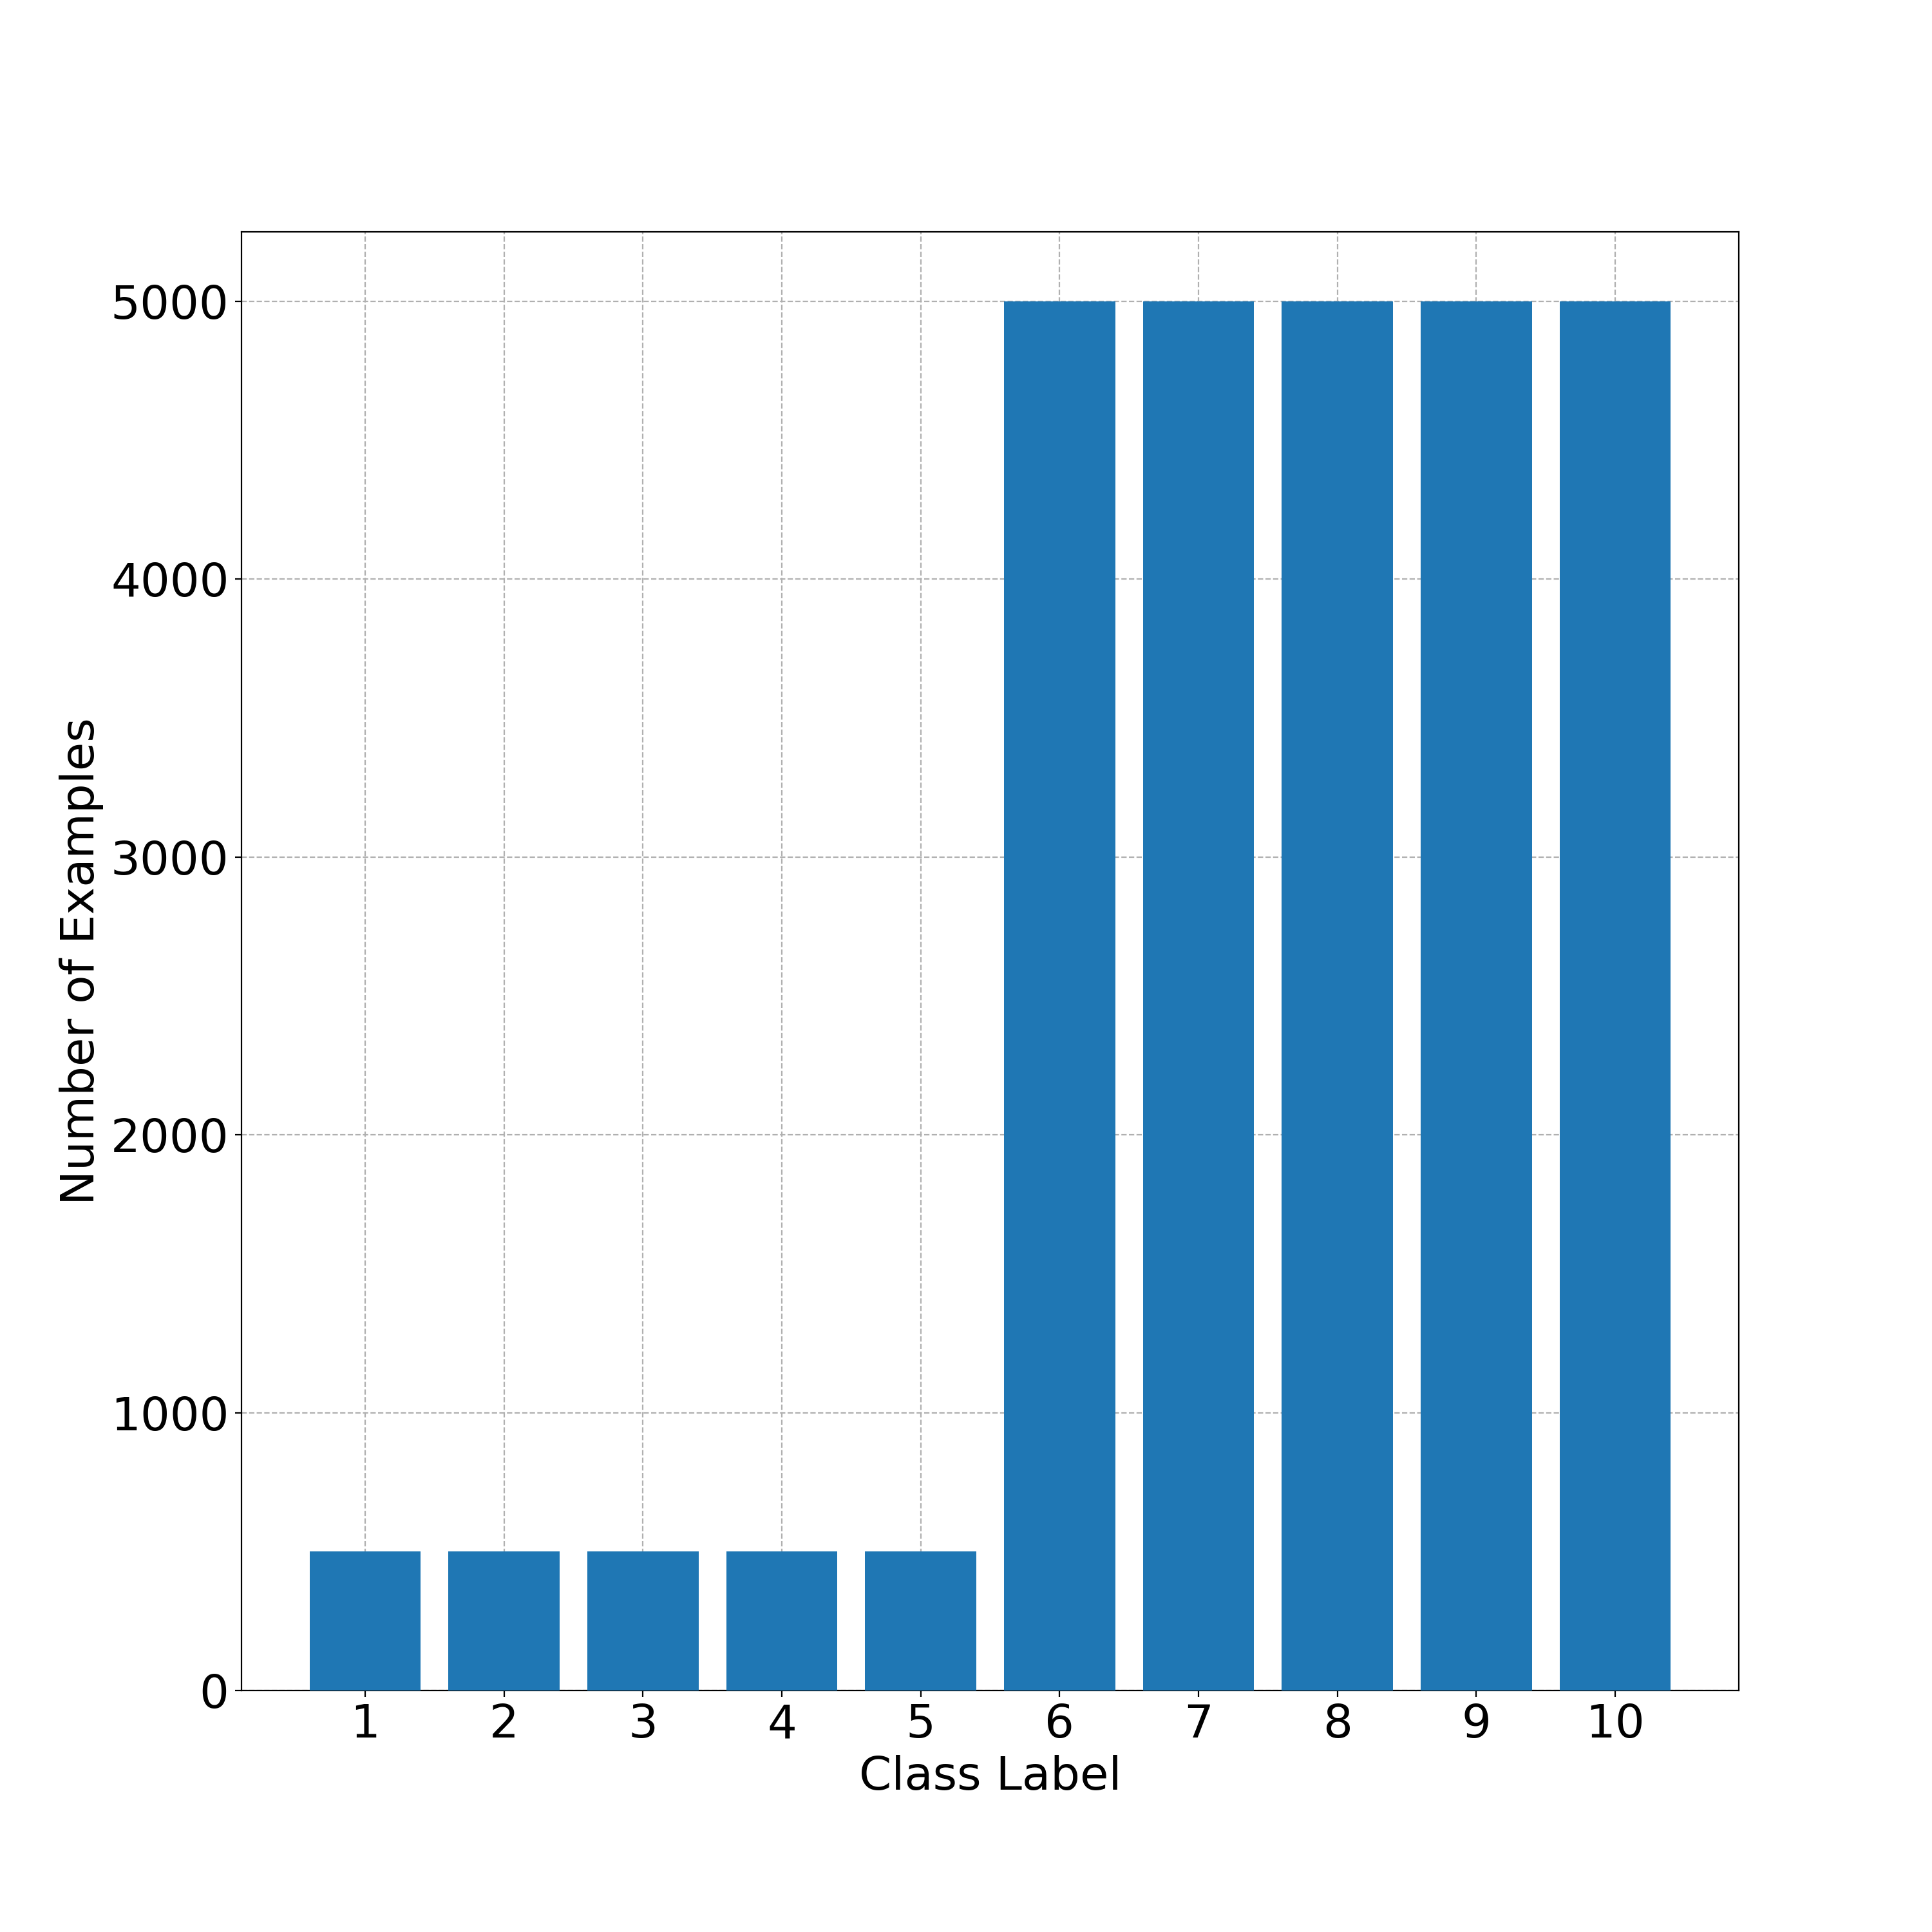
\includegraphics[width=0.45\columnwidth]{imbalance-distribution-1}
      \label{fig:imb-dist:1}
  }
  \subfigure[]{
      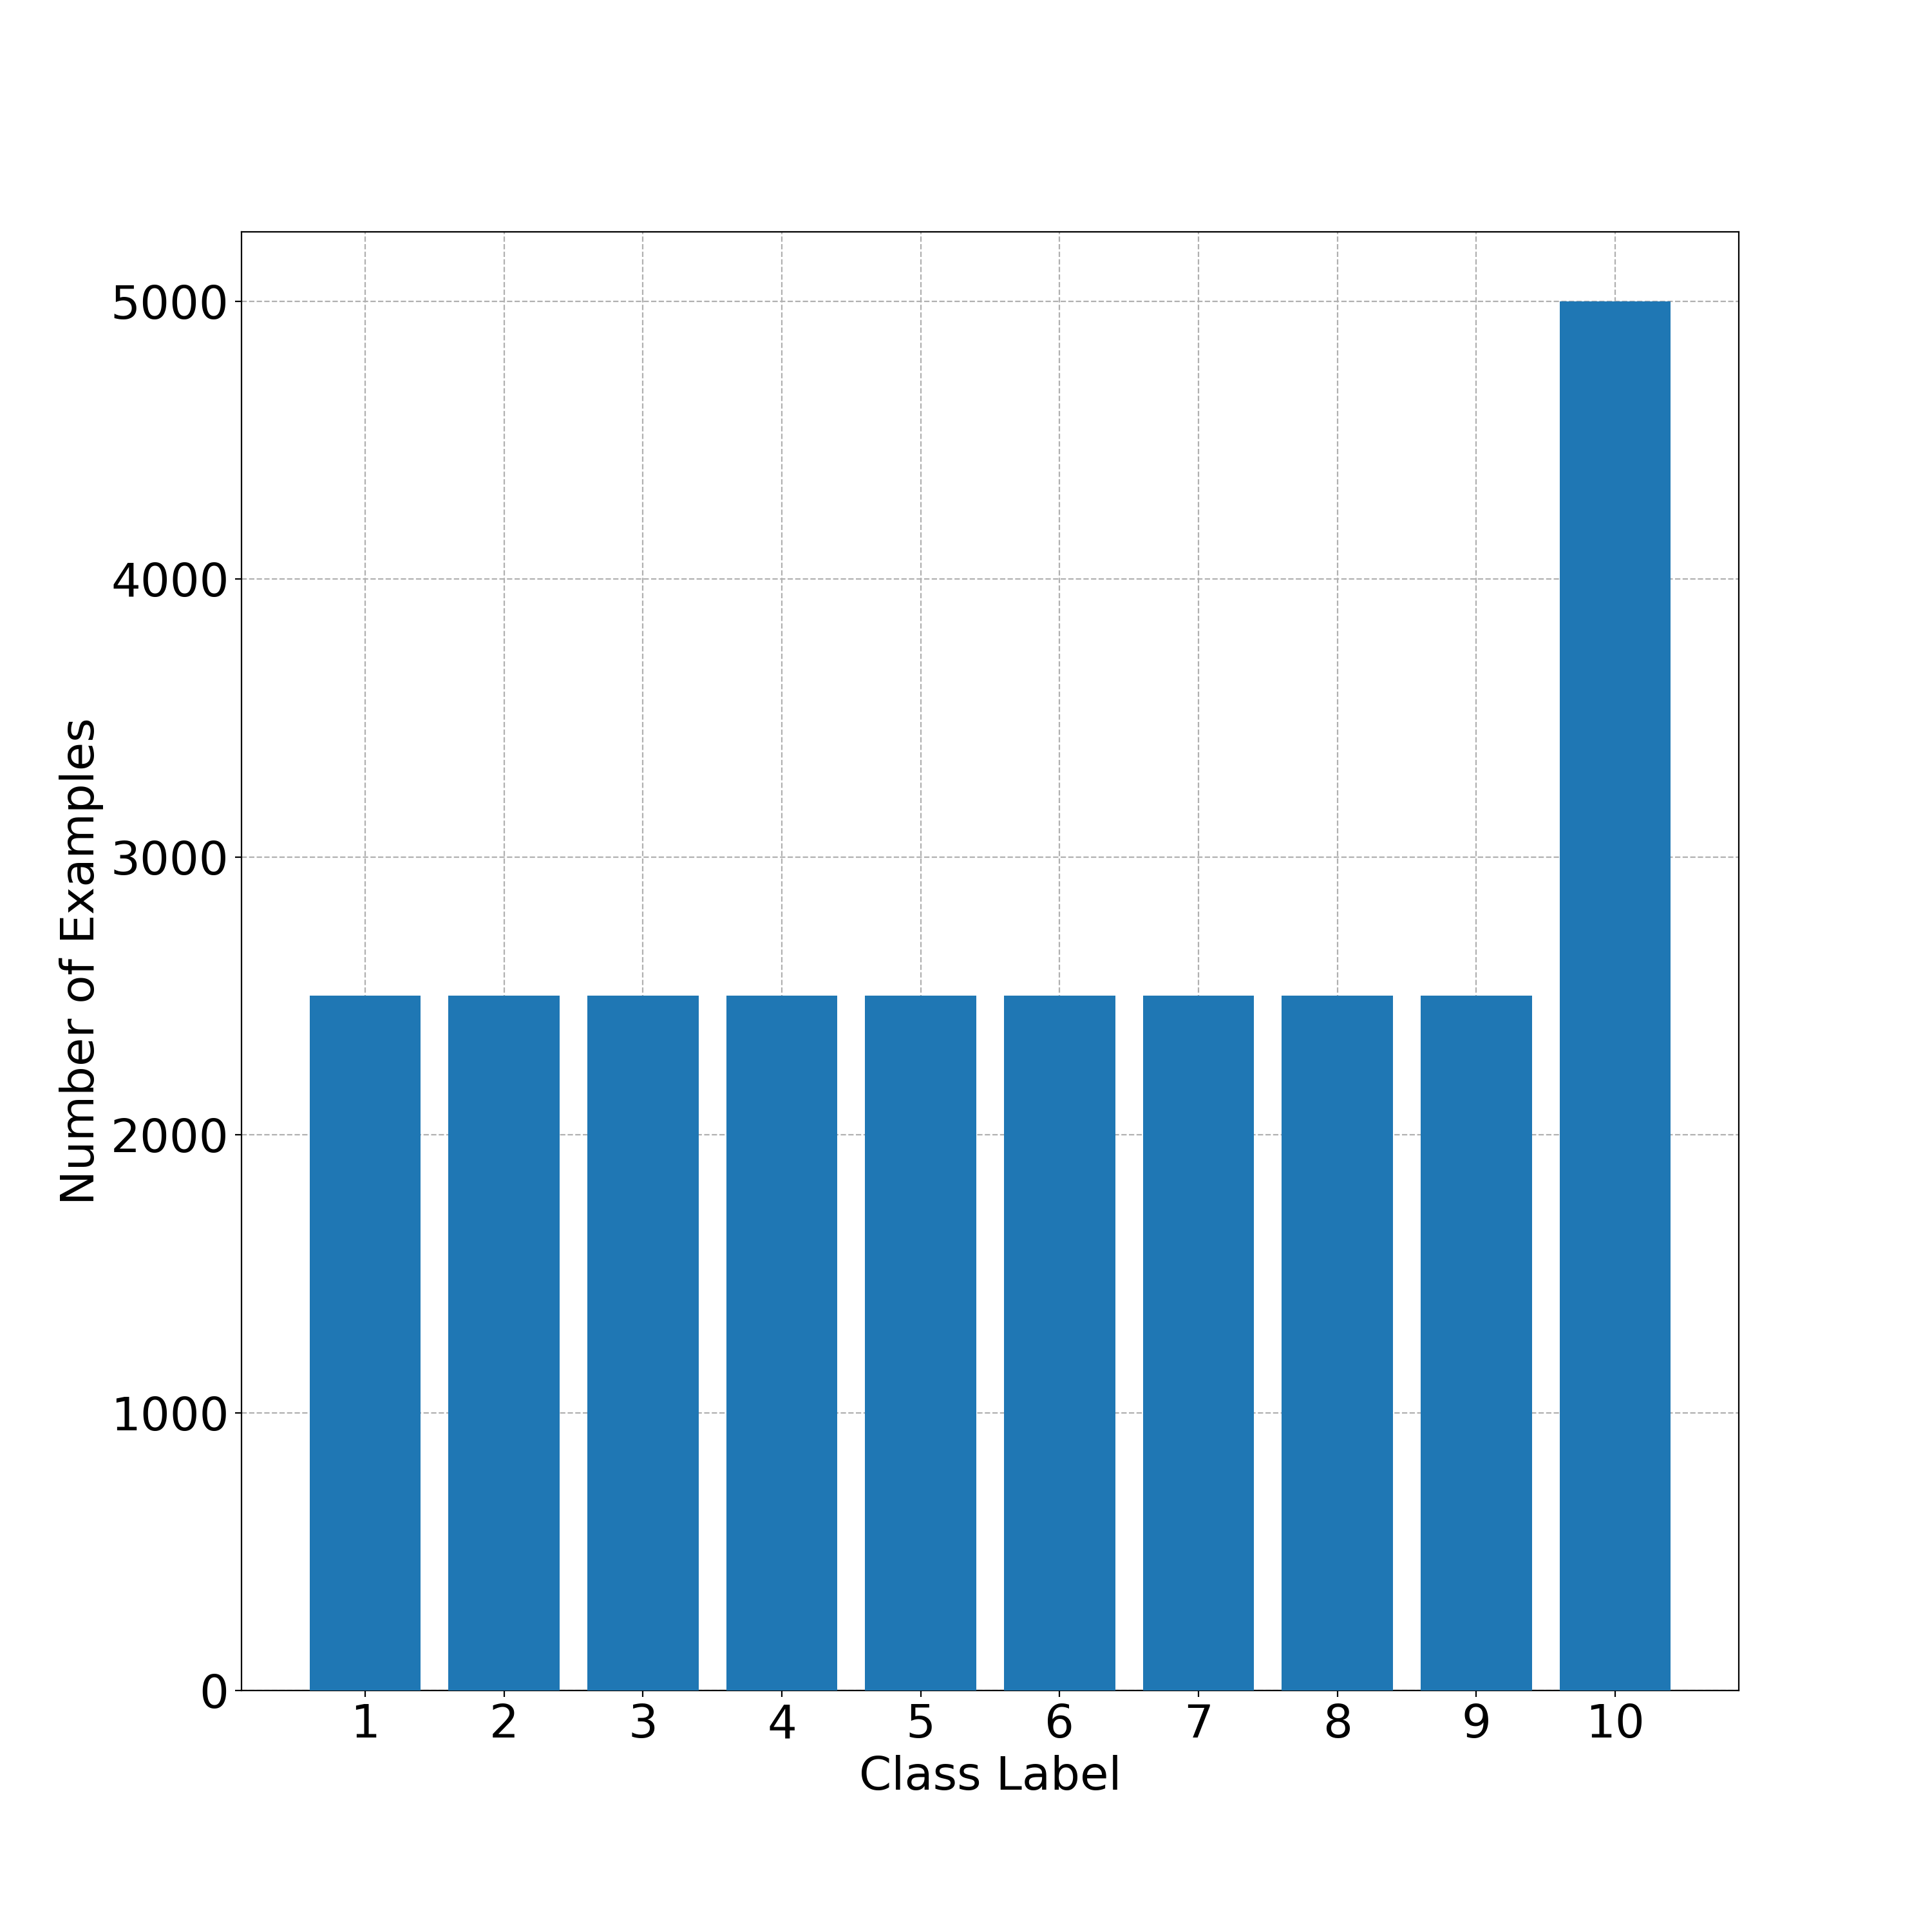
\includegraphics[width=0.45\columnwidth]{imbalance-distribution-2}
      \label{fig:imb-dist:2}
  }
  \subfigure[]{
    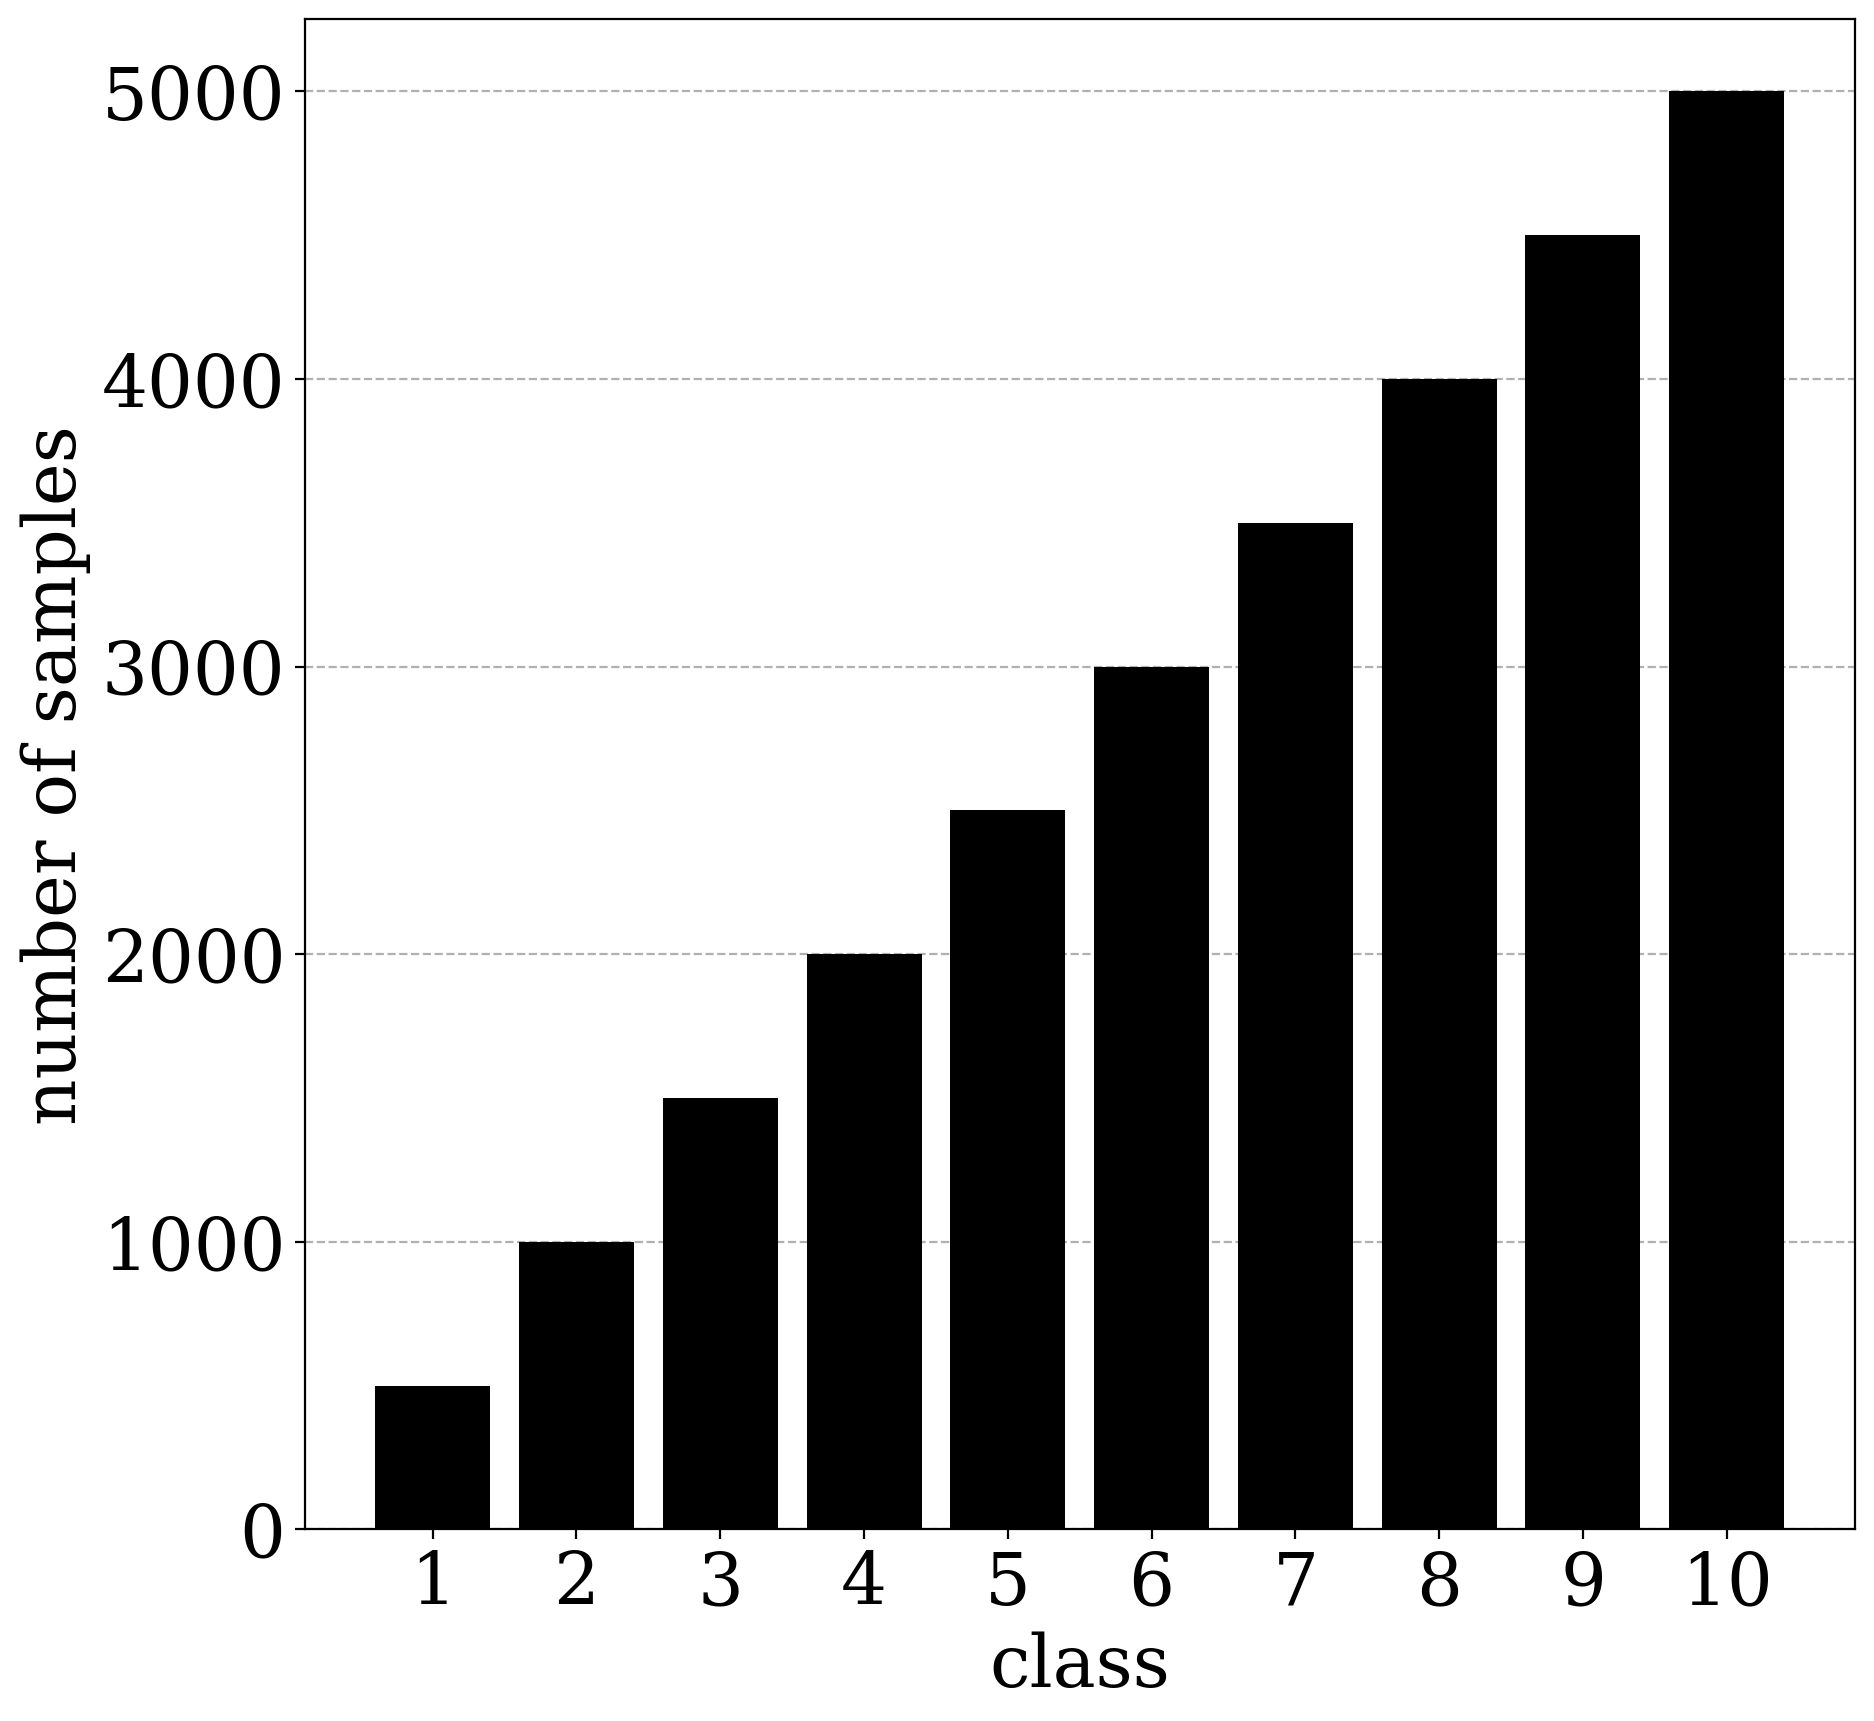
\includegraphics[width=0.45\columnwidth]{imbalance-distribution-3}
    \label{fig:imb-dist:3}
  }
  \caption{ตัวอย่างการกระจายของจำนวนตัวอย่างของกลุ่มข้อมูล (ก) $p = 10$, $\mu = 0.5$ (ข) $p = 2$, $\mu = 0.9$ (ค) $p = 10$}
  \label{fig:imb-dist}
\end{figure}
\FloatBarrier

เพื่อที่จะพิสูจน์ว่าวิธีการที่นำเสนอในงานวิจัยนี้นั้นมีประสิทธิภาพ ในเบื้องต้นจะมุ่งศึกษาที่การจัดกลุ่มข้อมูลสองกลุ่ม ที่ซึ่งลักษณะของความไม่สมดุลกันจะเป็นแบบ Step Imbalance และในอนาคตจะทำการพิสูจน์วิธีการที่นำเสนอกับการจัดกลุ่มข้อมูลหลายกลุ่ม โดยในรายงานฉบับนี้จะขอกล่าวถึงกลุ่มข้อมูลส่วนมากว่า Negative Class และกลุ่มข้อมูลส่วนน้อยว่า Positive Class

\section{ฟังก์ชันสูญเสีย (Loss Function)}
ในกระบวนการเรียนรู้ของแบบจำลอง DNN ฟังก์ชันสูญเสียจะถูกใช้ในการคำนวณค่าสูญเสีย เพื่อนำไปปรับค่า Weight ของแบบจำลอง เมื่อค่าสูญเสียยิ่งมาก ค่า Weight จะถูกปรับจากค่าเดิมมาก ในทางเดียวกันถ้าค่าสูญเสียน้อย ค่า Weight จะถูกปรับจากค่าเดิมน้อยเช่นกัน หรือก็คือแบบจำลองเริ่มไม่เรียนรู้อะไรเพิ่มเติมแล้ว ดังนั้นค่าสูญเสียต้องเป็นค่าที่เหมาะสมให้มากที่สุด ไม่เช่นนั้นจะทำให้การปรับค่า Weight ของแบบจำลองเกิดการคลาดเคลื่อนได้ อย่างไรก็ตามปัญหานี้จะพบได้ในเฉพาะการเรียนรู้ของแบบจำลองกับข้อมูลที่ไม่สมดุล ดังตัวอย่างการคำนวณค่าสูญเสียใน~\cite{Wang:2016} โดยที่จำนวนตัวอย่างของกลุ่มข้อมูลส่วนมากและส่วนน้อยเท่ากับ 90 และ  10 ตัวอย่างตามลำดับ และแบบจำลองทำนายข้อมูลของกลุ่มข้อมูลส่วนมากผิดไป 4 ตัวอย่าง และสำหรับกลุ่มข้อมูลส่วนน้อยผิดไป 5 ตัวอย่าง ถ้าคำนวณค่าสูญเสียด้วย Mean Squared Error (MSE) จะได้ค่าสูญเสียเท่ากับ 0.09 ซึ่งจากค่าสูญเสียดังกล่าว มันไม่สมเหตุสมผลเลยที่ค่าสูญเสียจะน้อยขนาดนี้ เพราะแบบจำลองทำนายข้อมูลของกลุ่มข้อมูลส่วนน้อยผิดไปตั้งครึ่งหนึ่ง ด้วยเหตุนี้ทำให้ในการเรียนรู้ของแบบจำลองในรอบถัดไป ถูกกำหนดให้เปลี่ยนแปลงค่า Weight ไม่มาก ดังนั้นจากปัญหาที่กล่าวมาจำเป็นจะต้องมีฟังก์ชันสูญเสียที่สามารถคำนวณค่าสูญเสียได้อย่างสมเหตุสมผลที่สุด เพื่อให้การเรียนรู้ของแบบจำลองนั้นมีประสิทธิภาพ